\chapter{直流-交流変換 ― インバータ}
\label{chap9}

前章までの直流-直流変換と交流-直流変換に続き，本章では直流から交流を作り出す
\index{ちょくりゅうこうりゅうへんかん@直流-交流変換}\textbf{直流-交流変換}（DC-AC変換）を扱う。
この変換を行う回路を\index{いんばーた@インバータ}\textbf{インバータ}（inverter）という。
太陽電池やバッテリーが生み出すのは直流であり，一方でモータや送電網が求めるのは交流である。
その橋渡しをするインバータは，電気自動車の駆動，太陽光発電の系統連系，無停電電源装置（UPS）など，
現代の電力システムのいたるところで働いている。

\begin{screen}
\noindent\textbf{本章の現在地}\\[3pt]
序章の電力変換の地図（\ref{fig0.1}）の「直流→交流」に入る（9章）。
これまでの章がインダクタやキャパシタに\textbf{蓄えて放出する}比率で電圧を作り替えてきたのに対し，
本章の骨組みはもっと単純である ― \textbf{スイッチで直流電源の$+$と$-$を負荷に交互につなぎ替え，交流の骨組みを作る}。
そのままでは角ばった方形波にすぎないが，スイッチの切替えを細かく刻む\textbf{PWMで正弦波を彫り出し}，
最後に\textbf{4章のLCフィルタで磨けば}なめらかな交流になる。本章はこの3段構えを順にたどる。
\end{screen}

%%======================================================================
\section{ハーフブリッジ回路とフルブリッジ回路}
\label{sec9.1}

\subsection{交流は$+$と$-$を交互に出せばよい}

直流から交流を作る原理は拍子抜けするほど単純である。
負荷にかかる電圧の向きを，スイッチで周期的に反転させればよい。
前半の半周期は負荷に$+$の電圧を，後半の半周期は$-$の電圧を与えれば，
角ばってはいるが正負に振動する立派な交流 ― \index{ほうけいは@方形波}\textbf{方形波}が得られる。

この向きの反転を，直流電圧源とスイッチだけで実現する回路の基本形が2つある。
\index{はーふぶりっじ@ハーフブリッジ}\textbf{ハーフブリッジ}回路と
\index{ふるぶりっじ@フルブリッジ}\textbf{フルブリッジ}回路である（\FIGref{fig9.1}）。
まず回路の呼び名を整理しておく。

\begin{定義}[アーム・レグ・ブリッジ]
\label{def9.1}
上側または下側のスイッチ1つを\index{あーむ@アーム}\textbf{アーム}（arm），
上下のアームを直列にした縦1列を\index{れぐ@レグ}\textbf{レグ}（leg），
複数のレグで構成される回路全体を\index{ぶりっじ@ブリッジ}\textbf{ブリッジ}（bridge）という。
\end{定義}

\begin{figure}[ht]
\begin{center}
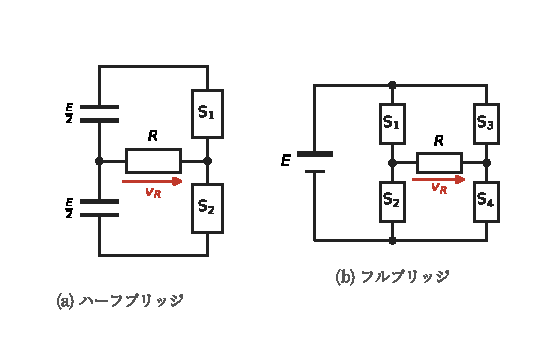
\includegraphics[clip]{figures/fig9.1.eps}
\end{center}
\caption{インバータの基本回路。(a)ハーフブリッジは1レグ（スイッチ2個）で構成し，
分割した電源の中点を基準に$\pm E/2$を出力する。(b)フルブリッジは2レグ（スイッチ4個）で構成し，
1つの電源から$\pm E$を出力する}
\label{fig9.1}
\end{figure}

\textbf{ハーフブリッジ回路}（\ref{fig9.1}(a)）は，直流電源を2つに分けて中点を作り，
1つのレグ（$\mathrm{S}_1$，$\mathrm{S}_2$）で負荷の片端をつなぎ替える。
$\mathrm{S}_1$をオンにすれば負荷には$+E/2$，$\mathrm{S}_2$をオンにすれば$-E/2$がかかる。
スイッチは2個で済むが，出力電圧の振幅は電源電圧$E$の半分にとどまる。

\textbf{フルブリッジ回路}（\ref{fig9.1}(b)）は，2つのレグ（$\mathrm{S}_1$〜$\mathrm{S}_4$）で
負荷の両端をつなぎ替える。$\mathrm{S}_1$と$\mathrm{S}_4$をオンにすると負荷の左端が$+$，右端が$-$になって
$v_R = +E$，逆に$\mathrm{S}_2$と$\mathrm{S}_3$をオンにすると$v_R = -E$になる。
スイッチは4個必要だが，1つの電源で振幅$E$の交流が得られる。
どちらの回路も直流電圧源を交流に変換するので，
\index{でんあつがたいんばーた@電圧形インバータ}\textbf{電圧形インバータ}と呼ばれる。

\begin{注意}
本章の解析では，これまでの章と同様に理想スイッチ（オンで電圧降下ゼロ，オフで電流ゼロ）と
定常状態を仮定する。また電源電圧$E$は一定とし，出力の1周期を$T$，
その角周波数を$\omega = 2\pi/T$と書く。この$\omega$は出力交流の周波数（たとえば$50$\,Hz）に対応し，
スイッチングの周波数とは別物であることに注意してほしい。
\end{注意}

\subsection{抵抗負荷の波形}

もっとも単純な抵抗負荷から見ていく。フルブリッジで前半に$+E$，後半に$-E$を出力すると，
出力電圧$v_R$は振幅$E$の方形波になる（\FIGref{fig9.2}の1段目）。
抵抗負荷ではオームの法則$i_R = v_R/R$がそのまま成り立つから，
電流も電圧と同じ形・同じ位相の方形波になる（2段目）。
\begin{equation}
v_R =
\left\{
\begin{array}{ll}
+E & (0 \le t < T/2) \\
-E & (T/2 \le t < T)
\end{array}
\right.
\qquad
i_R = \frac{v_R}{R}
\label{eq9.1}
\end{equation}
抵抗負荷では電圧と電流が同相で，話はここで終わる。
しかし実際のインバータがつながる相手はモータのような\textbf{誘導性負荷}であり，そこでは事情が一変する。

%%======================================================================
\section{デッドタイムと還流ダイオード}
\label{sec9.2}

\subsection{誘導性負荷では電流が遅れる}

モータの巻線のように，負荷がインダクタンス$L$をもつとどうなるか。
4章で学んだとおり，インダクタの電流は電圧を積分した形になり，急には変われない。
方形波電圧$\pm E$を印加すると，$v_L = L\,di/dt$より電流は
\begin{equation}
\frac{di}{dt} = \frac{v_L}{L}
\label{eq9.2}
\end{equation}
にしたがって直線的に増減し，電流波形は\textbf{三角波}状になる（\ref{fig9.2}の3段目）。
純粋なインダクタなら電圧が$+E$の半周期で傾き$E/L$で増え，$-E$の半周期で同じ傾きで減る。
実際のRL負荷では時定数$\tau = L/R$で指数関数状に変化し，\textbf{電流の位相が電圧より遅れる}。

\begin{figure}[ht]
\begin{center}
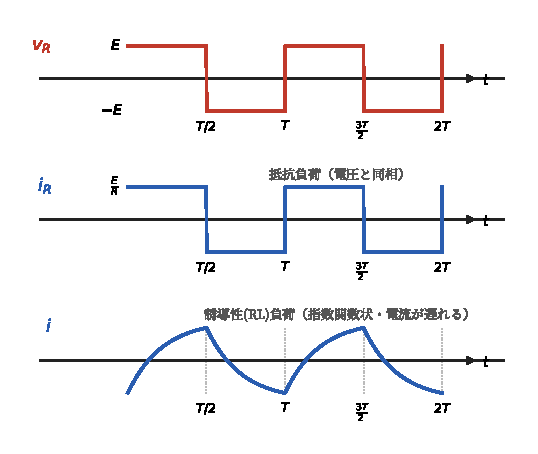
\includegraphics[clip]{figures/fig9.2.eps}
\end{center}
\caption{フルブリッジインバータの出力波形。抵抗負荷では電流$i_R$は電圧$v_R$と同相の方形波だが，
誘導性(RL)負荷では電流$i$は指数関数状になり，電圧に対して位相が遅れる}
\label{fig9.2}
\end{figure}

ここで重要なのは，電流が遅れる結果，\textbf{電圧を切り替えた直後もしばらく前と同じ向きの電流が流れ続ける}ことである。
たとえば$v_R$を$+E$から$-E$へ切り替えた瞬間，電流$i$はまだ$+$のまま流れている。
インダクタが磁場に蓄えたエネルギーを放出しようとするからで，この電流を
\index{かんりゅうでんりゅう@還流電流}\textbf{還流電流}（freewheeling current）という。
還流電流の行き場を用意しないと，インバータは壊れてしまう。その事情を次に見る。

\subsection{アーム短絡と同時オフの危険}

1つのレグの上下のスイッチ（たとえば$\mathrm{S}_1$と$\mathrm{S}_2$）が
\textbf{同時にオン}になると，電源が直接短絡される。
これを\index{あーむたんらく@アーム短絡}\textbf{アーム短絡}（上下短絡）といい，
極めて大きな電流がスイッチに流れて素子を破壊する。理想的には上下を一瞬で切り替えたいが，
実際のスイッチはオフになるのに時間がかかるため，切替えの瞬間に上下がわずかでも重なると短絡してしまう。

では逆に，切替えのときに上下を\textbf{同時にオフ}にすればよいかというと，それも危険である。
誘導性負荷では還流電流が流れているから，すべてのスイッチをオフにすると電流の行き場が突然なくなる。
式\ref{eq9.2}で$di/dt$が急激に大きくなり，$v_L = L\,di/dt$が跳ね上がって過大な電圧（サージ）が発生し，これもまた素子を壊す。

\subsection{デッドタイムを設け，還流ダイオードで逃がす}

この2つの危険を同時に避けるのが，デッドタイムと還流ダイオードの組合せである。

\begin{定義}[デッドタイム]
\label{def9.2}
1つのレグの上下のスイッチを切り替えるとき，アーム短絡を確実に防ぐために，
\textbf{両方をオフにする短い期間}を設ける。この期間を
\index{でっどたいむ@デッドタイム}\textbf{デッドタイム}（dead time）$t_d$という。
\end{定義}

デッドタイムを設ければアーム短絡は防げる（\FIGref{fig9.3}(a)）。
しかしデッドタイム中は上下ともオフだから，還流電流の行き場を別に用意しなければならない。
そこで各スイッチに逆向きの\index{かんりゅうだいおーど@還流ダイオード}\textbf{還流ダイオード}
（フリーホイールダイオード）を並列に接続する。
還流電流はこのダイオードを通って流れ続け，電流の連続性が保たれる（\ref{fig9.3}(b)）。
MOSFETの場合は構造上そなわっている\index{ぼでぃだいおーど@ボディダイオード}\textbf{ボディダイオード}
（寄生ダイオード）をそのまま還流ダイオードとして使えることが多い。

\begin{figure}[ht]
\begin{center}
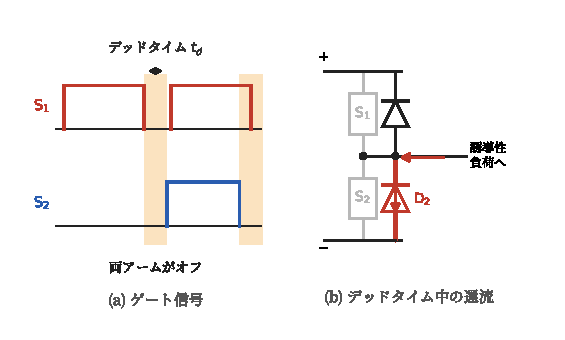
\includegraphics[clip]{figures/fig9.3.eps}
\end{center}
\caption{(a)上下アームのゲート信号。切替えのたびに両方がオフのデッドタイム$t_d$を挟む。
(b)デッドタイム中，誘導性負荷の還流電流は下アームの還流ダイオード$\mathrm{D}_2$を通って流れ続ける}
\label{fig9.3}
\end{figure}

\begin{例題}[デッドタイム時間の見積り]
\label{rei9.1}
あるMOSFETは，オフ信号を与えてから実際に電流を遮断し終えるまでの時間（ターンオフ時間）が
$t_{\mathrm{off}} = 200$\,ns，ゲート駆動回路の伝搬遅れのばらつきが$\pm 100$\,nsであるとする。
アーム短絡を防ぐのに必要なデッドタイム$t_d$を見積もれ。また，搬送波周波数
$f_c = 20$\,kHzで動作させるとき，デッドタイムが原因で失われる出力電圧はおよそ何\,\%か。
\begin{解答}
上アームがオフし終える前に下アームがオンし始めると短絡するから，
デッドタイムはターンオフ時間と遅れのばらつきの和より長くしなければならない。
余裕を$100$\,ns見込むと
\begin{equation*}
t_d \gtrsim t_{\mathrm{off}} + 100\,\mathrm{ns} + 100\,\mathrm{ns}
= 400\,\mathrm{ns}
\end{equation*}
となるので，$t_d = 0.5\,\mathrm{\mu s}$と選ぶ。
搬送波の1周期$T_c = 1/f_c = 50\,\mathrm{\mu s}$のうち，
上下の切替えは1周期に2回起こり，そのたびに$t_d$の間は出力が定まらない。
失われる時間の割合は
\begin{equation*}
\frac{2 t_d}{T_c} = \frac{2 \times 0.5}{50} = 0.02
\end{equation*}
すなわち出力電圧の基本波はおよそ$2$\,\%小さくなる。
デッドタイムは短いほどよいが，短くしすぎると短絡する。ここに設計の綱引きがある。
\end{解答}
\end{例題}

\begin{注意}
デッドタイム中の出力電圧は，そのとき流れている電流の向きに引きずられて決まる
（還流ダイオードがどちらのレールにつながるかで$+E$か$-E$のどちらかに張り付く）。
このため出力波形は指令からわずかにひずみ，低次の高調波を生む。これを
\textbf{デッドタイムひずみ}といい，正弦波を精密に作りたい用途では補正が行われる。
\end{注意}

\begin{問}
\item フルブリッジインバータで$E = 100$\,V，抵抗負荷$R = 10\,\Omega$のとき，
出力電圧$v_R$と電流$i_R$の波形の振幅を求めよ。次に負荷を誘導性(RL)に替えると，
電流波形の形と位相はどう変わるか，言葉で説明せよ。
\item 誘導性負荷で$v_R$を$+E$から$-E$へ切り替えた直後，電流$i$はまだ$+$の向きに流れている。
このときデッドタイム中に電流が通るのは，フルブリッジの4つの還流ダイオードのうちどれとどれか。
\ref{fig9.1}(b)を見て考えよ。
\end{問}

%%======================================================================
\section{フーリエ級数による出力波形の理解}
\label{sec9.3}

\subsection{方形波はいくつの正弦波でできているか}

インバータが出したいのは，本当はなめらかな正弦波である。
ところが方形波は角ばっている。この「ずれ」を正確にとらえる道具が
\index{ふーりえきゅうすう@フーリエ級数}\textbf{フーリエ級数}である。
周期$T$のどんな周期波形$v(t)$も，基本波（角周波数$\omega$）とその整数倍の角周波数をもつ
正弦波・余弦波の和で表せる。
\begin{equation}
v(t) = A_0 + \sum_{n=1}^{\infty}\left(A_n \cos n\omega t + B_n \sin n\omega t\right)
\label{eq9.3}
\end{equation}
$n=1$の項を\index{きほんは@基本波}\textbf{基本波}，$n \ge 2$の項を
\index{こうちょうは@高調波}\textbf{高調波}（$n$次高調波）という。
係数$A_n$，$B_n$は，「求めたい成分の波を掛けて1周期にわたって平均する」ことで取り出せる。
$\sin n\omega t$どうし，$\cos n\omega t$どうしは次数が同じときだけ平均が残り，異なる次数どうしや$\sin$と$\cos$の積は平均するとゼロになる（正弦波の直交性）。この性質を使うと
\begin{equation}
A_n = \frac{2}{T}\int_0^T v(t)\cos n\omega t\,dt,
\qquad
B_n = \frac{2}{T}\int_0^T v(t)\sin n\omega t\,dt
\label{eq9.4}
\end{equation}
となる。$A_n$，$B_n$は各成分の\textbf{振幅（ピーク値）}を表す。

\subsection{方形波のフーリエ係数を求める}

フルブリッジの出力（式\ref{eq9.1}）は，前半で$+E$，後半で$-E$をとる方形波である。
この波形は原点について点対称（奇関数）だから，余弦成分は含まれず$A_n = 0$である。
実際に式\ref{eq9.4}で計算してみよう。まず係数$B_n$を，半周期ごとに積分を分けて書く。
\begin{equation}
B_n = \frac{2}{T}\left[\int_0^{T/2} E \sin n\omega t\,dt
+ \int_{T/2}^{T}(-E)\sin n\omega t\,dt\right]
\label{eq9.5}
\end{equation}
$\int \sin n\omega t\,dt = -\dfrac{1}{n\omega}\cos n\omega t$を使って，途中を省かずに計算する。
\begin{eqnarray}
B_n &=& \frac{2E}{T}\left[
\left(-\frac{\cos n\omega t}{n\omega}\right)_0^{T/2}
- \left(-\frac{\cos n\omega t}{n\omega}\right)_{T/2}^{T}\right] \nonumber\\
&=& \frac{2E}{n\omega T}\left[
-\left(\cos\frac{n\omega T}{2} - 1\right)
+\left(\cos n\omega T - \cos\frac{n\omega T}{2}\right)\right]
\label{eq9.6}
\end{eqnarray}
ここで$\omega = 2\pi/T$だから$n\omega T = 2\pi n$，$n\omega T/2 = \pi n$である。
$\cos 2\pi n = 1$，$\cos \pi n = (-1)^n$を代入すると
\begin{eqnarray}
B_n &=& \frac{2E}{2\pi n}\left[
-\left((-1)^n - 1\right) + \left(1 - (-1)^n\right)\right] \nonumber\\
&=& \frac{E}{\pi n}\left[2 - 2(-1)^n\right]
= \frac{2E}{\pi n}\left[1 - (-1)^n\right]
\label{eq9.7}
\end{eqnarray}
となる。$1 - (-1)^n$は，$n$が偶数のとき$0$，奇数のとき$2$である。したがって
\begin{equation}
B_n =
\left\{
\begin{array}{ll}
\dfrac{4E}{\pi n} & (n = 1, 3, 5, \dots) \\[6pt]
0 & (n = 2, 4, 6, \dots)
\end{array}
\right.
\label{eq9.8}
\end{equation}
すなわち方形波は奇数次の正弦波だけでできており，
\begin{equation}
v_R(t) = \frac{4E}{\pi}\left(\sin\omega t + \frac{1}{3}\sin 3\omega t
+ \frac{1}{5}\sin 5\omega t + \cdots\right)
\label{eq9.9}
\end{equation}
と展開できる。基本波，3次，5次，$\dots$を足し合わせると，しだいに方形波に近づいていく（\FIGref{fig9.4}）。
各成分の振幅は次数$n$に反比例して小さくなり，方形波は基本波を主成分とすることがわかる。

\begin{figure}[ht]
\begin{center}
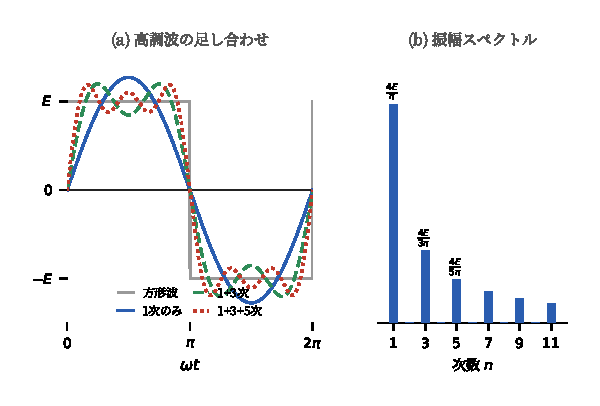
\includegraphics[clip]{figures/fig9.4.eps}
\end{center}
\caption{(a)基本波・3次・5次を足し合わせると方形波に近づく。
(b)高調波の振幅スペクトル。奇数次だけが現れ，振幅は$4E/(n\pi)$で$1/n$に減っていく}
\label{fig9.4}
\end{figure}

\subsection{基本波の振幅と実効値}

インバータが負荷に届けたいのは基本波である。式\ref{eq9.9}より，方形波に含まれる基本波の振幅は
\begin{equation}
\hat{V}_1 = \frac{4E}{\pi} \approx 1.27\,E
\label{eq9.10}
\end{equation}
であり，その実効値は
\begin{equation}
V_1 = \frac{\hat{V}_1}{\sqrt{2}} = \frac{4E}{\pi\sqrt{2}}
= \frac{2\sqrt{2}}{\pi}E \approx 0.90\,E
\label{eq9.11}
\end{equation}
となる。方形波全体の実効値は$E$だから，そのうち約$90$\,\%が基本波，残りが高調波である。
高調波の多さの目安を\index{ぜんこうちょうはひずみ@全高調波ひずみ}\textbf{全高調波ひずみ}
（THD：total harmonic distortion）で表すと，方形波では
\begin{equation}
\mathrm{THD} = \frac{\sqrt{E^2 - V_1^{2}}}{V_1}
= \frac{\sqrt{1 - 0.90^2}}{0.90} \approx 0.48
\label{eq9.12}
\end{equation}
すなわち約$48$\,\%にもなる。方形波のままでは高調波が多すぎて，モータのうなりや発熱の原因になる。
そこで次節以降の\textbf{振幅の制御}と\textbf{PWM}によって，基本波を目的の大きさに保ちつつ高調波を減らしていく。

\begin{例題}[高調波の振幅と実効値]
\label{rei9.2}
$E = 100$\,Vのフルブリッジ方形波インバータについて，
基本波・3次・5次高調波の振幅と，基本波の実効値を求めよ。
\begin{解答}
式\ref{eq9.8}より各高調波の振幅は
\begin{equation*}
\hat{V}_1 = \frac{4 \times 100}{\pi} \approx 127\,\mathrm{V},\quad
\hat{V}_3 = \frac{\hat{V}_1}{3} \approx 42\,\mathrm{V},\quad
\hat{V}_5 = \frac{\hat{V}_1}{5} \approx 25\,\mathrm{V}
\end{equation*}
基本波の実効値は式\ref{eq9.11}より
\begin{equation*}
V_1 = \frac{127}{\sqrt{2}} \approx 90\,\mathrm{V}
\end{equation*}
である。3次高調波は基本波の$1/3$，5次は$1/5$の振幅をもつことが確かめられる。
\end{解答}
\end{例題}

\begin{問}
\item 方形波の3次高調波と5次高調波の振幅は，基本波の振幅の何\,\%か。
また，基本波の実効値$V_1$が式\ref{eq9.11}のとおり全体の実効値$E$の約$90$\,\%になることを確かめよ。
\end{問}

%%======================================================================
\section{パルス幅制御・位相シフト制御}
\label{sec9.4}

\subsection{出力の振幅をどう変えるか}

方形波インバータの出力振幅は電源電圧$E$で決まってしまい，そのままでは変えられない。
出力を大きくも小さくもしたいときはどうするか。
考え方は「$+E$を出す時間を短くし，あいだに$0$の期間を挟む」ことである。
半周期のあいだ$+E$を出しっぱなしにするのではなく，一部を$0$にして幅を狭めれば，
波形に含まれる基本波の振幅が小さくなる。これを
\index{ぱるすはばせいぎょ@パルス幅制御}\textbf{パルス幅制御}という。

フルブリッジでは，左右のレグの切替えのタイミングを時間$\mathit{\Delta}t$だけずらすことで，これを実現できる。
2つのレグが同時に切り替わらないため，出力$v_R$は$+E$，$0$，$-E$の3つの値をとり，
$\pm E$のパルスの幅が$\mathit{\Delta}t$だけ狭くなる。左右のレグの位相をずらすので
\index{いそうしふとせいぎょ@位相シフト制御}\textbf{位相シフト制御}ともいう。

このとき基本波の振幅がどうなるかは，フーリエ係数を計算すればわかる。
前節と同じ手順で係数$B_n$を求めると（詳しい計算は章末問題\ref{ex9.2}），
\begin{equation}
B_n = \frac{4E}{\pi n}\cos^2\!\left(\frac{n\omega \mathit{\Delta}t}{2}\right)
\label{eq9.13}
\end{equation}
となる。$\mathit{\Delta}t = 0$では$\cos^2 = 1$となって方形波（式\ref{eq9.8}）に一致し，
$\mathit{\Delta}t$を大きくするほど基本波の振幅
\begin{equation}
\hat{V}_1 = \frac{4E}{\pi}\cos^2\!\left(\frac{\omega \mathit{\Delta}t}{2}\right)
\label{eq9.14}
\end{equation}
は連続的に小さくなる。すなわち$\mathit{\Delta}t$という1つの量で出力の振幅を制御できる。
ずらす時間を変えるだけなので制御は簡単だが，方形波の親戚であることに変わりはなく，低次の高調波は多いままである。
高調波まで減らしたいなら，次節の正弦波PWMへ進む必要がある。

\begin{問}
\item 位相シフト制御で基本波の振幅を方形波の半分にしたい。式\ref{eq9.14}で
\begin{equation*}
\cos^2\!\left(\frac{\omega\mathit{\Delta}t}{2}\right) = \frac{1}{2}
\end{equation*}
となる$\mathit{\Delta}t$を，出力周期$T$を使って表せ。
\end{問}

%%======================================================================
\section{正弦波PWM}
\label{sec9.5}

\subsection{正弦波に合わせてパルス幅を刻む}

パルス幅制御を一歩進める。半周期に1個の幅広パルスを出すのではなく，
半周期を細かく分けて多数の細いパルスを出し，\textbf{そのパルス幅を正弦波の大きさに合わせて変える}。
正弦波が大きいところではパルスを太く，小さいところでは細くすれば，
パルスの「平均」が正弦波をなぞる。これが
\index{せいげんはPWM@正弦波PWM}\textbf{正弦波PWM}（sinusoidal PWM，パルス幅変調）である。

パルス幅を正弦波に合わせる仕掛けは巧妙で，2つの波を比較するだけでよい（\FIGref{fig9.5}(a)）。
1つは目標の正弦波である\index{へんちょうは@変調波}\textbf{変調波}（指令信号）$v_{\mathrm{ref}}$，
もう1つはそれよりずっと高い周波数の三角波である\index{はんそうは@搬送波}\textbf{搬送波}
（キャリア）$v_{\mathrm{carr}}$である。この2つを比べ，
\textbf{変調波が搬送波より大きい区間はスイッチをオン，小さい区間はオフ}にする。
すると自然に，正弦波が大きいところほどオンの時間が長い（パルスが太い）パルス列が得られる（\ref{fig9.5}(b)）。

\begin{figure}[ht]
\begin{center}
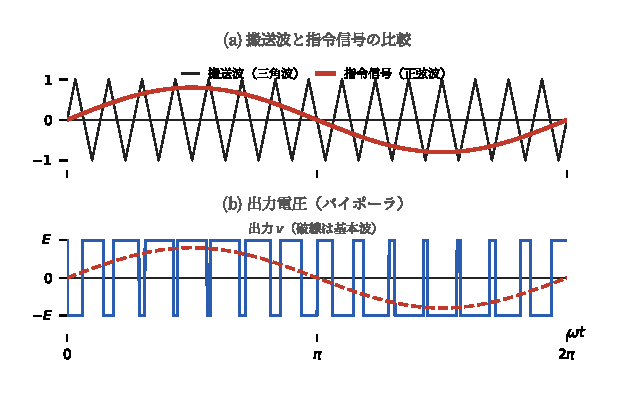
\includegraphics[clip]{figures/fig9.5.eps}
\end{center}
\caption{正弦波PWM（バイポーラ変調）。(a)正弦波の変調波と三角波の搬送波を比較する。
(b)変調波が搬送波を上回る区間で$+E$，下回る区間で$-E$を出力する。破線は取り出したい基本波}
\label{fig9.5}
\end{figure}

\subsection{変調率と基本波の振幅}

出力の基本波の大きさは，搬送波に対する変調波の大きさの比で決まる。

\begin{定義}[変調率]
\label{def9.3}
搬送波の振幅$\hat{v}_{\mathrm{carr}}$に対する変調波の振幅$\hat{v}_{\mathrm{ref}}$の比
\begin{equation}
m = \frac{\hat{v}_{\mathrm{ref}}}{\hat{v}_{\mathrm{carr}}}
\label{eq9.15}
\end{equation}
を\index{へんちょうりつ@変調率}\textbf{変調率}（変調度，modulation index）という。
\end{定義}

$0 \le m \le 1$の範囲では，出力電圧の基本波の振幅は変調率$m$に比例する。
ハーフブリッジ（出力$\pm E/2$）では，基本波の振幅は
\begin{equation}
\hat{V}_1 = m\,\frac{E}{2}
\qquad(0 \le m \le 1)
\label{eq9.16}
\end{equation}
となる（$E$は直流電源電圧）。フルブリッジ（出力$\pm E$）ならこの2倍で$\hat{V}_1 = mE$である。
$m$を$0$から$1$まで動かせば基本波の振幅を連続的に制御できるので，
\textbf{振幅は変調率で，周波数は変調波の周波数で}別々に決められる。これが正弦波PWMの強みである。

\begin{注意}
$m > 1$にすると，変調波の山が搬送波の頂点を越え，そこではパルスが途切れずオンのままになる。
これを\index{かへんちょう@過変調}\textbf{過変調}という。基本波はもう$m$に比例して増えず，出力に低次の高調波が混じり始める。
$m = 1$を超えて出力を増やすと，究極的には方形波（基本波振幅$4E/\pi$）に行き着く。
線形に制御できるのは$m \le 1$の範囲である。
\end{注意}

\subsection{バイポーラ変調とユニポーラ変調}

正弦波PWMには，出力パルスの作り方で2つの方式がある。
これまで見てきたのは，出力が$+E$と$-E$の2値を行き来する
\index{ばいぽーらへんちょう@バイポーラ変調}\textbf{バイポーラ変調}である。
一方，フルブリッジの左右のレグを別々の指令（$+v_{\mathrm{ref}}$と$-v_{\mathrm{ref}}$）で制御すると，
出力は$+E$，$0$，$-E$の3値をとる\index{ゆにぽーらへんちょう@ユニポーラ変調}\textbf{ユニポーラ変調}になる。

両者の違いは，発生する高調波の\textbf{周波数帯}にはっきり現れる（\FIGref{fig9.6}）。
どちらも基本波（低い周波数）はきれいに取り出せるが，PWMが生む高調波は搬送波周波数の付近に集まる。
バイポーラでは搬送波周波数$f_c$（次数$m_f$）の付近に，
ユニポーラでは左右のレグが交互に切り替わるため実効的なスイッチング周波数が2倍になり，
高調波は$2f_c$（次数$2m_f$）の付近に移る。
高調波がより高い周波数へ押しやられるので，ユニポーラのほうが同じ搬送波周波数でも高調波が少なく，
後段のLCフィルタ（4章）で取り除くのも容易である。

\begin{figure}[ht]
\begin{center}
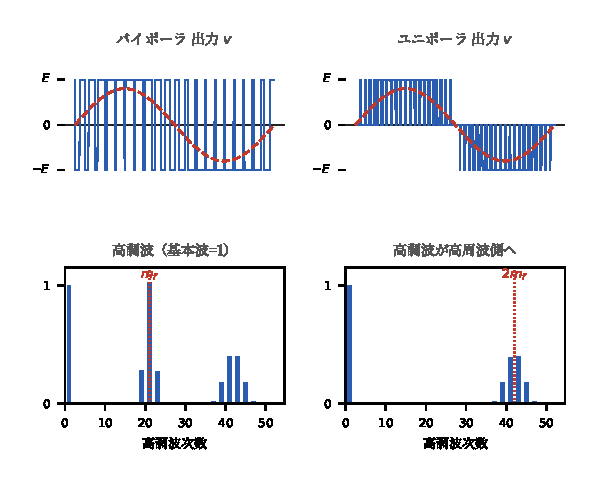
\includegraphics[clip]{figures/fig9.6.eps}
\end{center}
\caption{バイポーラ変調とユニポーラ変調の出力波形（上）と高調波スペクトル（下）。
高調波は基本波付近には現れず搬送波周波数の付近に集まる。
ユニポーラでは実効スイッチング周波数が2倍になり，高調波が$2m_f$付近のより高い周波数帯へ移る}
\label{fig9.6}
\end{figure}

高調波が搬送波付近の高い周波数に固まってくれるのは大きな利点である。
低い周波数の基本波と，高い周波数の高調波とは，カットオフ周波数をその間に置いたLCローパスフィルタで
きれいに切り分けられる。搬送波周波数を高くするほど高調波はさらに高い周波数へ逃げ，
必要なフィルタのインダクタ・キャパシタは小さくて済む（\ref{sec5.8}節の高周波化と同じ理屈である）。

\begin{例題}[変調率と基本波の振幅]
\label{rei9.3}
直流電源$E = 200$\,Vのハーフブリッジインバータを，変調率$m = 0.8$の正弦波PWMで動かす。
出力電圧の基本波の振幅と実効値を求めよ。また，同じ電源のフルブリッジをバイポーラ変調で
$m = 0.8$で動かすと基本波の振幅はいくらか。
\begin{解答}
ハーフブリッジは式\ref{eq9.16}より
\begin{equation*}
\hat{V}_1 = m\,\frac{E}{2} = 0.8 \times \frac{200}{2} = 80\,\mathrm{V}
\end{equation*}
実効値は$V_1 = 80/\sqrt{2} \approx 57\,\mathrm{V}$である。
フルブリッジではこの2倍で$\hat{V}_1 = mE = 0.8 \times 200 = 160\,\mathrm{V}$となる。
同じ電源でもフルブリッジは2倍の振幅が得られることがわかる。
\end{解答}
\end{例題}

\begin{問}
\item ハーフブリッジ正弦波PWM（$E = 300$\,V）で，基本波の実効値を$100$\,Vにしたい。
必要な変調率$m$を求めよ。この$m$は線形制御の範囲（$m \le 1$）に収まっているか。
\end{問}

%%======================================================================
\section{マルチレベルインバータ}
\label{sec9.6}

\subsection{段数を増やして正弦波に近づける}

これまでの回路は，出力が$\pm E$（フルブリッジ）や$0, \pm E$（ユニポーラ）といった
少数の電圧レベルしかとれなかった。1回のスイッチングで電圧が$E$も跳ぶため，
高調波が大きく，また急峻な電圧変化$dv/dt$がノイズ（11章）の原因にもなる。
さらに，オフのスイッチには電源電圧$E$がまるごとかかるので，高耐圧の素子が必要になる。

そこで，出力がとれる電圧レベルの\textbf{段数を増やす}のが
\index{まるちれべるいんばーた@マルチレベルインバータ}\textbf{マルチレベルインバータ}である。
たとえば電源を2つに分けて中点を作り，出力に$0$，$\pm E/2$，$\pm E$といった中間レベルを加えると，
出力は正弦波をなめらかな\textbf{階段波}で近似できる（\FIGref{fig9.7}）。
段数が増えるほど1段の高さが小さくなり，正弦波との差（＝高調波）が減る。

\begin{figure}[ht]
\begin{center}
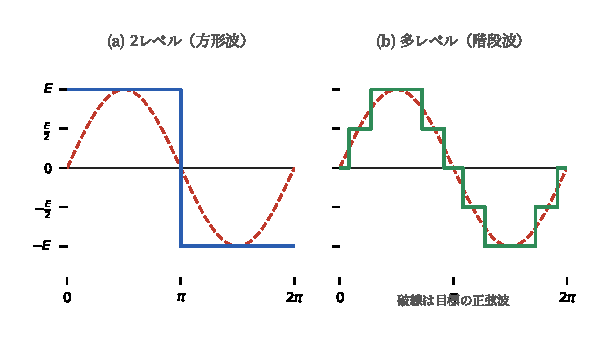
\includegraphics[clip]{figures/fig9.7.eps}
\end{center}
\caption{(a)2レベルの方形波と，(b)多レベルの階段波。破線の目標正弦波に対し，
段数を増やすほど階段が細かくなって正弦波に近づき，高調波が減る}
\label{fig9.7}
\end{figure}

中間レベルを作る代表的な回路が
\index{ちゅうせいてんくらんぷ@中性点クランプ}\textbf{中性点クランプ}方式（NPC：neutral-point-clamped）である。
分割した電源の中点を，クランプダイオードを介して出力につなぐことで，
1つのレグで$0$，$E/2$，$E$の3レベルを出せる。マルチレベルインバータの利点は3つある。
(1)~出力が正弦波に近く高調波が少ない，(2)~1回のスイッチングの電圧の跳びが$E/2$と小さく$dv/dt$による
ノイズが減る，(3)~オフのスイッチにかかる電圧が$E/2$で済むので素子の耐圧を下げられる。
これらの理由から，高電圧・大電力のインバータでは多レベル化が広く使われている。

\begin{問}
\item 3レベル（中性点クランプ）方式のインバータで，オフになっているスイッチにかかる電圧は
電源電圧$E$の何分の1か。この方式が高電圧のインバータで好まれる理由を，素子の耐圧の観点から説明せよ。
\end{問}

%%======================================================================
\section{ゲート駆動回路}
\label{sec9.7}

\subsection{スイッチを速く確実にオン・オフする}

ここまでスイッチは理想的に一瞬で切り替わるとしてきたが，
実際にMOSFETをオン・オフさせるには専用の回路がいる。それが
\index{げーとくどうかいろ@ゲート駆動回路}\textbf{ゲート駆動回路}（ゲートドライバ）である。

MOSFETのゲートは，絶縁膜をはさんだ導体であり，電気的には\textbf{キャパシタ}とみなせる。
オンにするには，このゲートのキャパシタに電荷をためて，しきい値以上の電圧をかけなければならない。
オンにするのに必要な電荷を\index{げーとでんか@ゲート電荷}\textbf{ゲート電荷}$Q_g$といい，
データシートに記載されている。素早くオンにするには，短い時間で$Q_g$を送り込む
＝\textbf{大きな電流を一瞬だけ流す}必要がある。マイコンの出力ピンでは電流が足りないため，
大電流を供給できる\index{げーとどらいば@ゲートドライバ}\textbf{ゲートドライバ}
（プッシュプル回路，トーテムポール回路）を間に入れる。

速く切り替えることは損失の面でも重要である。スイッチの切替えの途中は，
電圧と電流がともにゼロでない状態を通るため，その積である電力が失われる。これを
\index{すいっちんぐそんしつ@スイッチング損失}\textbf{スイッチング損失}という（3章）。
切替えを速くすればこの中間状態が短くなり，1回あたりの損失が減る。
ゲートドライバで大電流を流して切替えを速くするのは，そのためでもある。

\subsection{ハイサイド駆動とブートストラップ}

ここで1つ厄介な問題が起こる。ハーフブリッジの下アーム（ローサイド）のMOSFETは，
ソースがグラウンドに固定されているので駆動しやすい。
ところが上アーム（\index{はいさいど@ハイサイド}\textbf{ハイサイド}）のMOSFETは，
そのソースがレグの中点につながっており，スイッチングのたびに電位が$0$と$E$のあいだで大きく上下する。
ゲートはソースを基準にして$+$の電圧をかける必要があるから，
\textbf{浮動する基準電位の上に，もう1つの電源}を用意しなければならない。

この浮いた電源を安く実現するのが
\index{ぶーとすとらっぷ@ブートストラップ}\textbf{ブートストラップ}回路である（\FIGref{fig9.8}）。
ハイサイド用のキャパシタ$C_{boot}$を1個追加し，
下アーム$\mathrm{Q}_2$がオンでレグ中点がほぼグラウンド電位にある間に，
制御電源$V_{cc}$からダイオード$\mathrm{D}_{boot}$を通して$C_{boot}$を充電しておく。
上アーム$\mathrm{Q}_1$を駆動するときは，充電された$C_{boot}$が中点電位の上に乗った電源として働き，
ハイサイドのゲートに電荷を供給する。$\mathrm{Q}_2$がオンになるたびに充電が繰り返されるので，
1個のキャパシタとダイオードだけでハイサイド電源をまかなえる。

\begin{figure}[ht]
\begin{center}
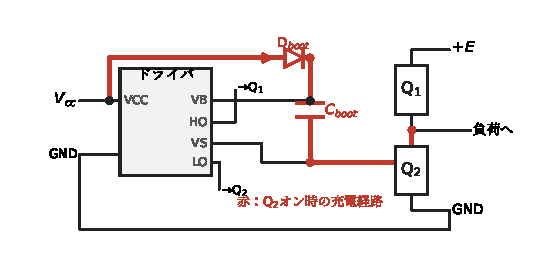
\includegraphics[clip]{figures/fig9.8.eps}
\end{center}
\caption{ブートストラップによるハイサイド駆動。下アーム$\mathrm{Q}_2$がオンの間に，
$V_{cc}$から$\mathrm{D}_{boot}$を通して$C_{boot}$を充電する（赤の経路）。
充電された$C_{boot}$が，浮動する中点電位$V_S$の上に乗ったハイサイド用電源として働く}
\label{fig9.8}
\end{figure}

\begin{注意}
ブートストラップ方式では，下アームがオンになる期間がないと$C_{boot}$を充電できない。
このため上アームを長時間オンにし続ける用途には向かず，起動時には最初に下アームをオンにして
$C_{boot}$を充電する手順が必要になる。
\end{注意}

\begin{問}
\item （単位検算）あるMOSFETのゲート電荷は$Q_g = 65$\,nCである。
これを$t = 100$\,nsでゲートに送り込むために必要な平均電流$I = Q_g/t$を求め，
右辺の単位が電流の単位A（アンペア）になることを確かめよ。
\end{問}

\subsection{本章のまとめと次章へ}

本章では，スイッチで直流電源の$+$と$-$を交互につなぎ替えて交流の骨組みを作り，
フーリエ級数で方形波を高調波に分解し，パルス幅制御と正弦波PWMで基本波の振幅を制御し，
マルチレベル化で高調波を減らす，という流れをたどった。
根っこにあるのは章頭で述べた3段構え ―
\textbf{スイッチで$\pm$を切り替え，PWMで正弦波を彫り出し，LCフィルタ（4章）で磨く}である。
生み出された高調波が搬送波周波数の付近に固まってくれるからこそ，
低い周波数の基本波だけをLCフィルタで取り出せるのであった。

こうして直流と交流を自在に行き来できるようになった。残るは交流を別の交流へ直接作り替える変換である。
交流→直流→交流と2段階を踏まずに，周波数や振幅を直接変換する ― それが次章の交流-交流変換である。

%%======================================================================
\begin{章末問題}
\item \label{ex9.1}フルブリッジ方形波インバータ（電源電圧$E$，出力周期$T$）の出力電圧のフーリエ級数を求めよう。
\begin{enumerate}
\item[(a)] 出力$v_R$（式\ref{eq9.1}）が奇関数であることから，余弦成分$A_n = 0$を説明せよ。
\item[(b)] 式\ref{eq9.5}から出発し，$B_n = \dfrac{2E}{\pi n}[1-(-1)^n]$（式\ref{eq9.7}）を途中を省かずに導け。
\item[(c)] $E = 100$\,Vのとき，基本波・3次・5次高調波の振幅を求め，全高調波ひずみが約$48$\,\%になることを確かめよ。
\end{enumerate}

\item \label{ex9.2}位相シフト制御の出力波形は，$0 \le t < T/2 - \mathit{\Delta}t$で$+E$，
$T/2 \le t < T - \mathit{\Delta}t$で$-E$，それ以外で$0$をとる。
\begin{enumerate}
\item[(a)] フーリエ係数が
\begin{equation*}
B_n = \frac{2}{T}\left[\int_0^{T/2-\mathit{\Delta}t}E\sin n\omega t\,dt
+ \int_{T/2}^{T-\mathit{\Delta}t}(-E)\sin n\omega t\,dt\right]
\end{equation*}
で与えられることを確かめよ。
\item[(b)] これを計算し，$B_n = \dfrac{4E}{\pi n}\cos^2\!\left(\dfrac{n\omega\mathit{\Delta}t}{2}\right)$
（式\ref{eq9.13}）を導け。$1+\cos\theta = 2\cos^2(\theta/2)$を使ってよい。
\item[(c)] 基本波の振幅を方形波の$70$\,\%にするための$\mathit{\Delta}t$を，$T$を使って求めよ。
\end{enumerate}

\item \label{ex9.3}直流電源$E = 400$\,Vのフルブリッジインバータを正弦波PWM（バイポーラ変調）で動かす。
\begin{enumerate}
\item[(a)] 変調率$m = 0.9$のときの基本波の振幅と実効値を求めよ。
\item[(b)] 出力の基本波の実効値を$0$から最大まで連続的に変えたい。線形制御で得られる基本波実効値の最大値はいくらか。
\item[(c)] さらに出力を増やそうと$m$を$1$より大きくすると何が起こるか。過変調について説明せよ。
\end{enumerate}

\item \label{ex9.4}デッドタイムについて考える。あるインバータのMOSFETのターンオフ時間は$t_{\mathrm{off}} = 300$\,ns，
ゲート駆動の遅れのばらつきは$\pm 150$\,nsである。
\begin{enumerate}
\item[(a)] アーム短絡を防ぐのに必要なデッドタイム$t_d$を，余裕を$150$\,ns見込んで見積もれ。
\item[(b)] 搬送波周波数$f_c = 15$\,kHzのとき，デッドタイムのために失われる出力電圧の割合を求めよ。
\item[(c)] 搬送波周波数を$f_c = 60$\,kHzに上げると，この割合はどうなるか。
高周波化とデッドタイムの関係を説明せよ。
\end{enumerate}

\item \label{ex9.5}3レベル（中性点クランプ）方式のフルブリッジインバータでは，
各レグが$0$，$E/2$，$E$の3レベルを出せる。
\begin{enumerate}
\item[(a)] フルブリッジ全体で，出力$v_R$がとりうる電圧レベルをすべて挙げよ。
\item[(b)] 2レベルのフルブリッジと比べて，1回のスイッチングでの電圧の跳びは何分の1になるか。
\item[(c)] オフのスイッチにかかる電圧が$E/2$で済むことは，どんな利点につながるか。
高電圧インバータでの意義を述べよ。
\end{enumerate}

\item \label{ex9.6}（LTspiceで確かめよ）フルブリッジインバータを正弦波PWMで動かすモデルを作り，
次を確かめよ。負荷はRL直列（たとえば$R = 10\,\Omega$，$L = 10$\,mH），
搬送波$f_c = 5$\,kHz，変調波$50$\,Hz，変調率$m = 0.8$とする。
\begin{enumerate}
\item[(a)] バイポーラ変調で出力電圧$v$と負荷電流$i$の波形を観測し，電流が正弦波に近づくことを確かめよ。
\item[(b)] 出力電圧をFFTし，高調波が搬送波周波数$f_c$の付近に集まることを確かめよ。
\item[(c)] ユニポーラ変調に変えると，高調波の集まる周波数と負荷電流のリプルはどう変わるか。
バイポーラの結果と比較せよ（\ref{sec9.5}節の予想と照らし合わせよ）。
\item[(d)] 変調率$m$を$0.5$，$1.0$，$1.2$と変えて，基本波の振幅の変化を調べよ。
$m = 1.2$で線形の関係$\hat{V}_1 = mE$から外れる（過変調）ことを確かめよ。
\end{enumerate}
\end{章末問題}
